\documentclass[tikz,border=0pt]{standalone}
\usepackage[american]{circuitikz}
\usetikzlibrary{arrows.meta,calc,positioning,decorations.pathmorphing,patterns}
\definecolor{zyloTeal}{HTML}{174A5B}
\definecolor{zyloTealTwo}{HTML}{246B7A}
\definecolor{zyloInk}{HTML}{1F2933}
\definecolor{zyloSoft}{HTML}{EAF4F4}
\definecolor{zyloPaper}{HTML}{F8FAFB}
\definecolor{zyloLine}{HTML}{44606B}
\definecolor{zyloOrange}{HTML}{D97706}
\begin{document}
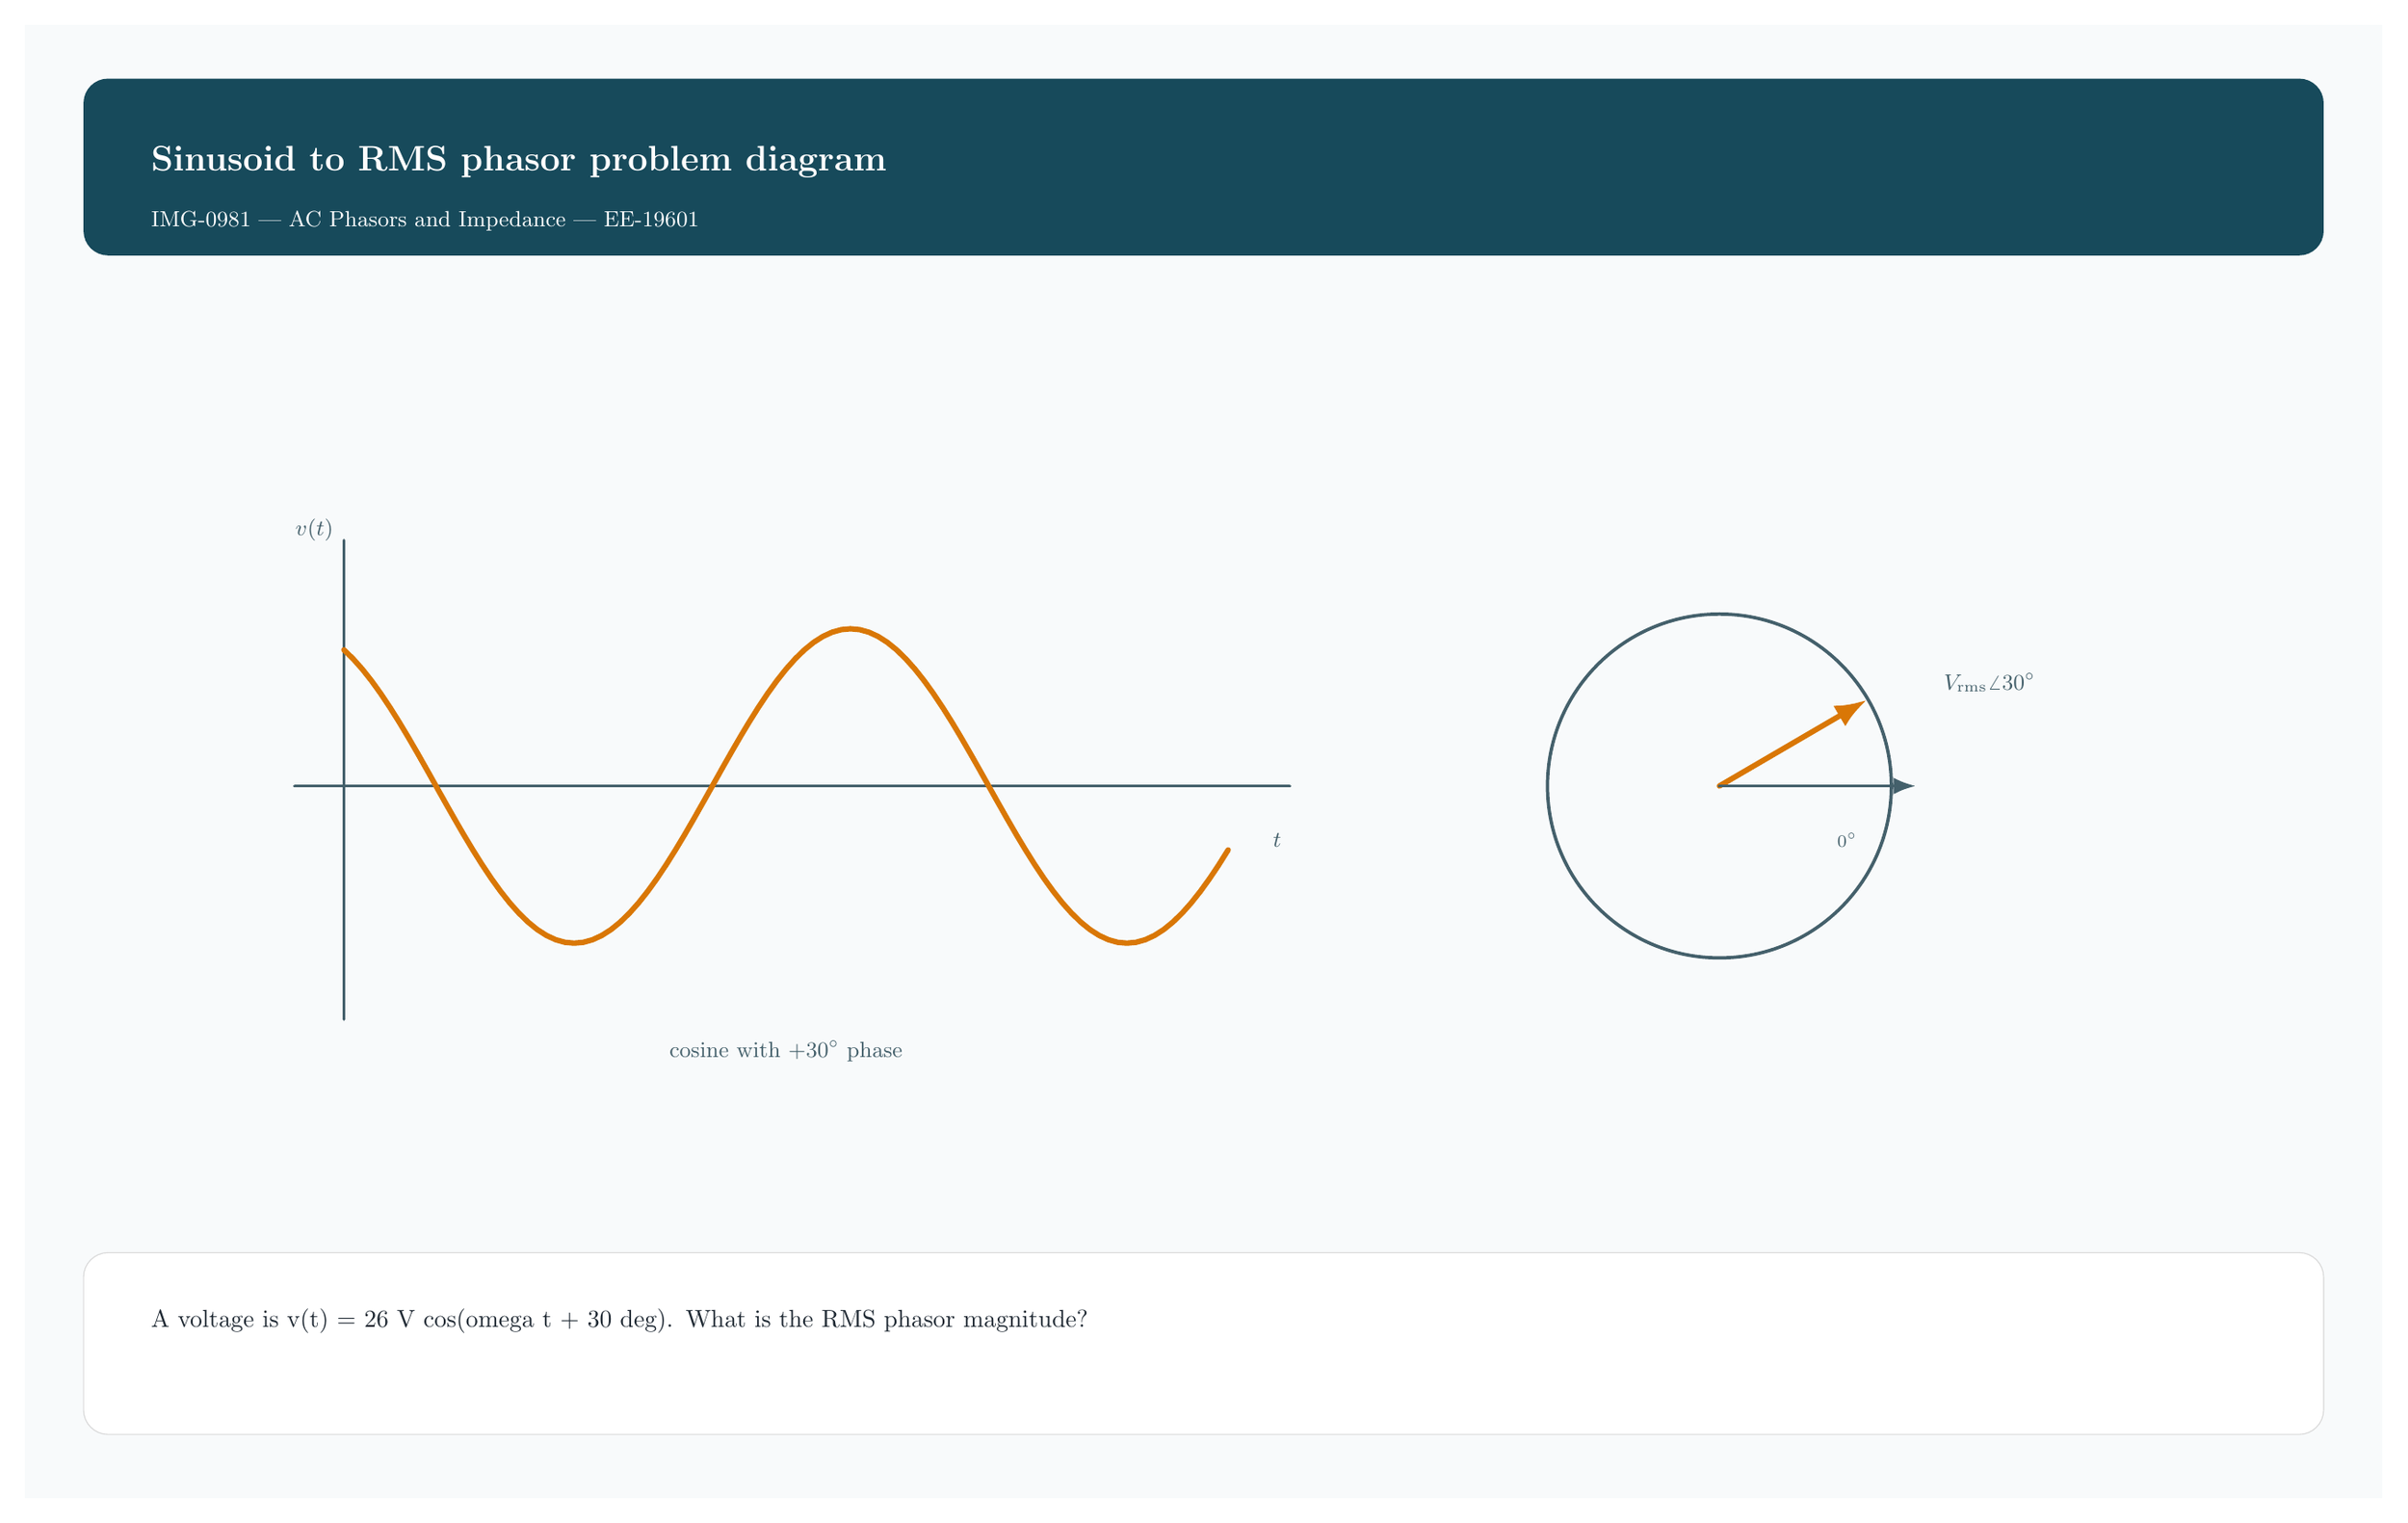
\begin{tikzpicture}[x=1pt,y=-1pt,>=Latex,line cap=round,line join=round]
\path[fill=zyloPaper] (0,0) rectangle (960,600);
\path[fill=zyloTeal,rounded corners=10pt] (24,22) rectangle (936,94);
\node[anchor=west,text=white,font=\bfseries\Large] at (48,56) {Sinusoid to RMS phasor problem diagram};
\node[anchor=west,text=white!82,font=\small] at (48,80) {IMG-0981 | AC Phasors and Impedance | EE-19601};
\tikzset{wire/.style={draw=zyloTeal,line width=2.2pt},thinwire/.style={draw=zyloLine,line width=1.35pt},accent/.style={draw=zyloOrange,line width=2.2pt},box/.style={draw=zyloTealTwo,fill=zyloSoft,line width=1.5pt,rounded corners=8pt}}
\draw[thinwire] (110,310) -- (515,310);
\draw[thinwire] (130,405) -- (130,210);
\draw[accent] (130,254.574) -- (133.75,258.223) -- (137.5,262.439) -- (141.25,267.176) -- (145,272.382) -- (148.75,278) -- (152.5,283.969) -- (156.25,290.223) -- (160,296.694) -- (163.75,303.31) -- (167.5,310) -- (171.25,316.69) -- (175,323.306) -- (178.75,329.777) -- (182.5,336.031) -- (186.25,342) -- (190,347.618) -- (193.75,352.824) -- (197.5,357.561) -- (201.25,361.777) -- (205,365.426) -- (208.75,368.467) -- (212.5,370.868) -- (216.25,372.601) -- (220,373.649) -- (223.75,374) -- (227.5,373.649) -- (231.25,372.601) -- (235,370.868) -- (238.75,368.467) -- (242.5,365.426) -- (246.25,361.777) -- (250,357.561) -- (253.75,352.824) -- (257.5,347.618) -- (261.25,342) -- (265,336.031) -- (268.75,329.777) -- (272.5,323.306) -- (276.25,316.69) -- (280,310) -- (283.75,303.31) -- (287.5,296.694) -- (291.25,290.223) -- (295,283.969) -- (298.75,278) -- (302.5,272.382) -- (306.25,267.176) -- (310,262.439) -- (313.75,258.223) -- (317.5,254.574) -- (321.25,251.533) -- (325,249.132) -- (328.75,247.399) -- (332.5,246.351) -- (336.25,246) -- (340,246.351) -- (343.75,247.399) -- (347.5,249.132) -- (351.25,251.533) -- (355,254.574) -- (358.75,258.223) -- (362.5,262.439) -- (366.25,267.176) -- (370,272.382) -- (373.75,278) -- (377.5,283.969) -- (381.25,290.223) -- (385,296.694) -- (388.75,303.31) -- (392.5,310) -- (396.25,316.69) -- (400,323.306) -- (403.75,329.777) -- (407.5,336.031) -- (411.25,342) -- (415,347.618) -- (418.75,352.824) -- (422.5,357.561) -- (426.25,361.777) -- (430,365.426) -- (433.75,368.467) -- (437.5,370.868) -- (441.25,372.601) -- (445,373.649) -- (448.75,374) -- (452.5,373.649) -- (456.25,372.601) -- (460,370.868) -- (463.75,368.467) -- (467.5,365.426) -- (471.25,361.777) -- (475,357.561) -- (478.75,352.824) -- (482.5,347.618) -- (486.25,342) -- (490,336.031);
\node[font=\small,text=zyloLine] at (118,206) {$v(t)$}; \node[font=\small,text=zyloLine] at (510,332) {$t$};
\node[font=\small,text=zyloLine] at (310,418) {cosine with $+30^\circ$ phase};
\draw[thinwire] (690,310) circle (70); \draw[accent,->] (690,310) -- (750,275); \draw[thinwire,->] (690,310) -- (770,310);
\node[font=\small,text=zyloLine] at (800,268) {$V_{\mathrm{rms}}\angle30^\circ$}; \node[font=\scriptsize,text=zyloLine] at (742,332) {$0^\circ$};
\path[draw=black!15,fill=white,rounded corners=10pt] (24,500) rectangle (936,574);
\node[anchor=west,text width=860pt,align=left,text=zyloInk,font=\normalsize] at (48,528) {A voltage is v(t) = 26 V cos(omega t + 30 deg). What is the RMS phasor magnitude?};
\end{tikzpicture}
\end{document}
